%!TEX root = main.tex

\section{Related work}

We structure the discussion of previous work into two categories:
related work on the estimation of user influence and
work concerning bot presence and behavior on Twitter.
%, applied to to the 2016 U.S. election.

\textbf{Estimating user influence on Twitter.}
Aggregate measures such as the follower count, the number of retweets and the number of mentions have been shown to be indicative of user influence on Twitter~\cite{Cha2010,kwak2010twitter}.
%Early attempts to estimate influence on Twitter used measures such as follower count, the number of rewteets and the number of mentions~\cite{Cha2010}. 
More sophisticated estimates of user influence use eigenvector centrality to account for the connectivity of followers or retweeters; 
for example, TwitteRank~\cite{twitterrank} extends PageRank~\cite{pagerank} by taking into account topical similarity between users and network structure.
Other extensions like Temporal PageRank~\cite{rozenshtein2016temporal} explicitly incorporate time into ranking to account for a time-evolving network.
%Further work attempted to control for the decay of influence over time~\cite{Mishra2016}, with Temporal PageRank~\cite{rozenshtein2016temporal} explicitly incorporating time in ranking. 
However, one limitation of PageRank-based methods is that they require a complete mapping of the social networks.
% (hence involving significant storage and computation).
% \TODO{MAR}{Whereas we are linear time and quadratic memory!}. 
More fundamentally, network centrality has the drawback of evaluating only the \textit{potential} of a user to be influential in spreading ideas or content, and it does not account for the actions of the user (e.g. tweeting on a particular subject).
%is a fairly ``blunt'' measure of influence: while, for example, a user with high centrality in a Twitter following network has the \textit{potential} to be influential in spreading ideas or content, it does not tell us 
%whether the user has undertaken any actions to actually achieved this influence. 
Our influence estimation approach proposed in Sec.~\ref{sec:user-influence} is built starting from the user Twitter activity and it does not require knowledge of the social network.

Recent work~\cite{ICWSM1613006,Chikhaoui:2017:DCA:3127339.3070658} has focused on estimating user influence as the contribution to information diffusion. 
For example, ConTinEst~\cite{Du2013} requires a complete diffusion graph and employs a random sampling algorithm to approximate user influence with scalable complexity.
However, constructing the complete diffusion graph might prove problematic, as current state-of-the-art methods for uncovering the diffusion structure (e.g. \cite{Gomez-Rodriguez2011,simma2012modeling,cho2013latent,li2013dyadic,linderman2014discovering}) do not scale to the number of users in our dataset. 
This is because these methods assume that a large number of cascades occur in a rather small social neighborhood, whereas in \debate cascades occur during a short period of time in a very large population of users.
%uses NetRate~\cite{Gomez-Rodriguez2011} to infer the social network underlying a large number of information diffusion cascades, employing a random sampling algorithm to approximate user influence with scalable complexity. 
%However, for the present paper, we do not have access to the large number of complete information cascades that are required for ConTinEst approach. 
Our proposed algorithm estimates influence directly from retweet cascades, without the need to reconstruct the retweet graph, and it scales cubically with the number of users.
%We therefore present and evaluate an innovative algorithm for estimating retweet diffusion-based user influence where there is incomplete cascade data.

%!TEX root = main.tex

\begin{figure*}[tbp]
	\newcommand\mywidth{0.19}
	\centering
	\subfloat[] {
		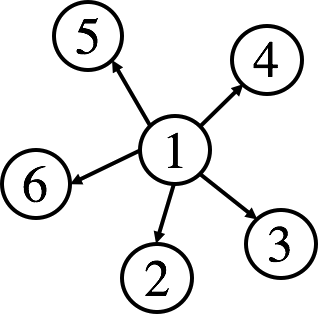
\includegraphics[width=0.14\textwidth,valign=c]{observcas}
		\vphantom{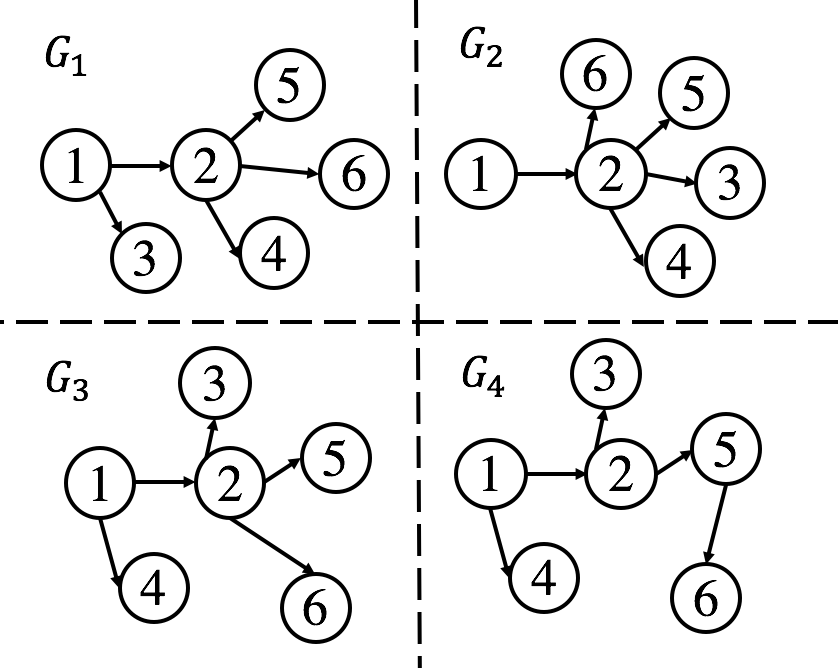
\includegraphics[height=\mywidth\textheight,valign=c]{somepossicas}}% MAR: this is here to keep the label at the same position as for the other figures.
		\label{fig:side:a}
	}
	\hspace{0.15cm}
	\subfloat[] {
		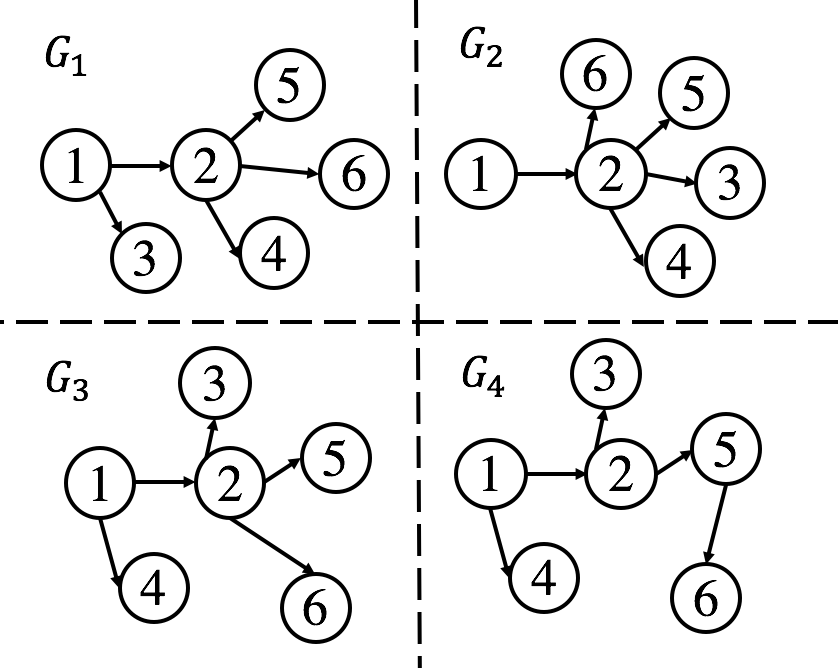
\includegraphics[height=\mywidth\textheight,valign=c]{somepossicas}
		\label{fig:side:b}
	}
	\hspace{0.15cm}
	\subfloat[] {
		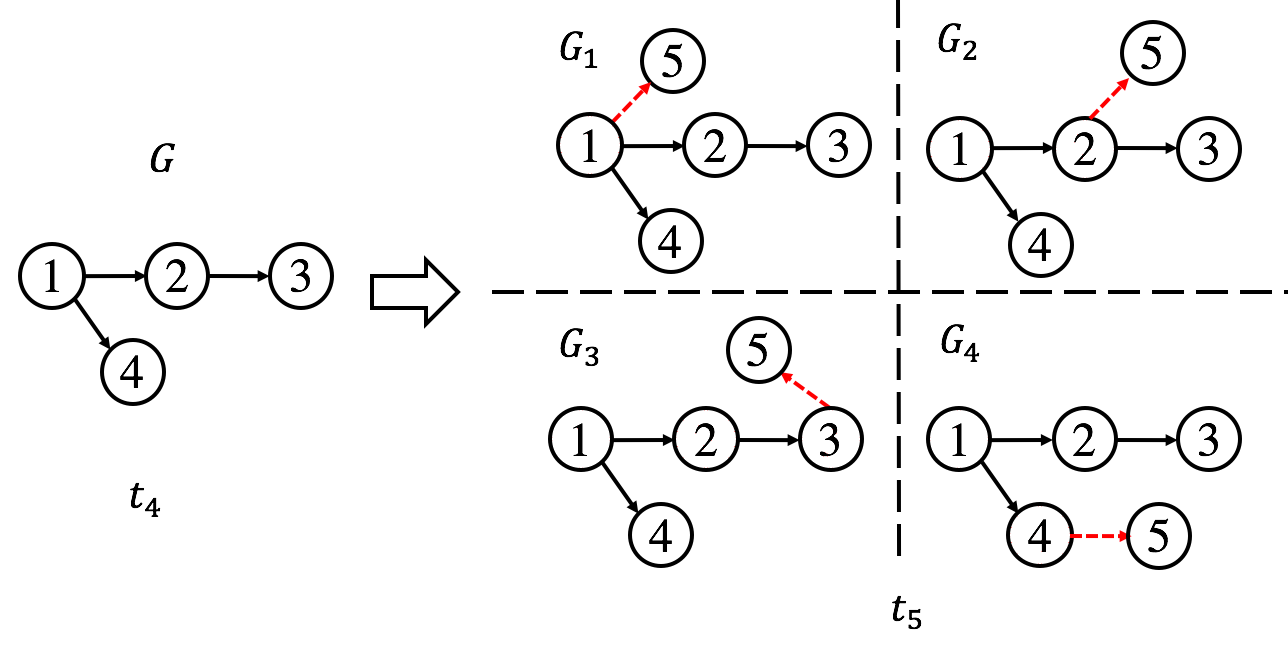
\includegraphics[height=\mywidth\textheight,valign=c]{gen_col}
		\label{fig:add-one-edge}
	}
	\caption{ 
		Modeling latent diffusions.
		\textbf{(a)} The schema of a retweet cascade as provided by the Twitter API, in which all retweets are attributed to the original tweet.
		\textbf{(b)} Four diffusion scenarios (out of 120 possible scenarios), associated with the retweet cascade in (a).
		\textbf{(c)} Intuition of the independent conditional model.
		A new node $v_5$ appears conditioned on one diffusion scenario $G$.
		Four new diffusion scenarios are generated as $v_5$ can attach to any of the existing nodes.
%		\hl{The influence of each of the nodes colored in red increases as $v_5$ attaches.}\verify{LX: unclear what ``increases'' refers to. suggest removing the red coloring and the sentence. i.e. this caption works equally well without the two highlighted sentences.}
	}
	\label{fig:holdout-ll}
%	\captionmoveup
\end{figure*}

%\subsection{Bot Presence and Behavior on Twitter During the 2016 U.S. presidential election}
\textbf{Bot presence and behavior on Twitter.}
\label{previousworkbots}
%
The `BotOrNot' Twitter bot detection API uses a Random Forest supervised machine learning classifier to calculate the likelihood of a given Twitter user being a bot, based on more than 1,000 features extracted from meta-data, patterns of activity, and tweet content (grouped into six main classes: user-based; friends; network; temporal; content and language; and sentiment) 
\cite{davisetal.16,varol.17}\footnote{See: \url{https://botometer.iuni.iu.edu/\#!/}}.
The bot scores are in the range $[0,1]$, where 0 (1) means the user is very unlikely (likely) to be a bot. 
%Evaluation against a publicly dataset of known Twitter bots demonstrated high accuracy and performance, and i
%It has been estimated that between 9\% and 15\% of active Twitter accounts are bots~\cite{varol.17}. 
BotOrNot was used to examine how socialbots affected political discussions on Twitter during the 2016 U.S. presidential election~\cite{FM7090}.
% collected data during all three presidential debates and the election period itself, resulting in a dataset of more than 20 million tweets by approximately 2.8 million unique user accounts authored between 16 September and 21 October 2016. The authors classified the top 50,000 accounts ranked by activity volume, accounting for 60\% of the overall conversation; accounts with a BotOrNot score higher than 0.5 were classed as bots and extrapolating from the sample to the entire population of accounts, 
They found that bots accounted for approximately 15 \% (400,000 accounts) of the Twitter population involved in election-related activity, and authored about 3.8 million (19 \%) tweets. 
However, \citet{FM7090} sampled the most active accounts, which could bias upwards their estimate of the presence of bots as activity volume is one of the features that is used by BotOrNot. 
They found that bots were just as effective as humans at \textit{attracting retweets} from humans. 
\citet{Woolley.2017} used BotOrNot to test 157,504 users randomly sampled from 1,798,127 Twitter users participating in election-related activity 
%during 1-11 Nov 
and found that over 10\% were bots. 
%with the same bot score threshold of 0.5
Here we use BotOrNot to classify \textit{all} 1.5 million users in our dataset to obtain a less biased approximation of their numbers and impact.
%rather than a random and/or purposive sample. 

Previous work has studied the political partisanship of Twitter bots.
\citet{Kollanyi.2016.presidentialdebate} analyzed candidate-oriented hashtag use during the 1st U.S. presidential debate and found that highly automated accounts (self-identified bots and/or accounts that post at least 50 times a day) were disproportionately pro-Trump.
% in terms of tweeting and retweeting  (e.g., \#MakeAmericaGreatAgain for Trump; \#ImWithHer for Clinton).
\citet{FM7090} also studied political partisanship by identifying five pro-Trump and four pro-Clinton hashtags and assigning users to a particular political faction.
% depending on which candidates hashtags were in the majority in the top 10 hashtags appearing in tweets by the user. 
The results suggested that both humans and bots were more pro-Trump in terms of hashtag partisanship.
%\TODO{@MAR}{In the paragraph below I have introduced some short statements that bridge the computer and social science parts of the paper, which also clarify or qualify our motivation for the study. Could you please check to make sure it's all technically correct?}
However, the above findings are limited to a comparison between humans and bots of frequency counts of tweets authored and retweets received, and they provide no insight into the importance of users in retweet diffusions. 
We overcome this limitation by modeling the latent structure of retweet diffusions and computing user influence over all possible scenarios.

%However, such findings concerning human and bot retweeting activity might be biased by the fact that the Twitter API does not allow direct observation of retweet cascades. 
%Analysis of retweets is effectively limited to frequency statistics of original tweets.
%and cannot determine whether a particular \textit{retweet} in the diffusion is the likely cause of a massive cascade.
%We overcome this limitation by modeling the latent structure of retweet diffusions and computing user influence over all possible scenarios.


% The working paper by \citet{Kollanyi.2016.presidentialdebate} analysed a sample of 4.5 million tweets collected around the time of the 1st U.S. presidential debate. A set of 52 election- and candidate-oriented hashtags (e.g., \#MakeAmericaGreatAgain for Trump; \#ImWithHer for Clinton) were used to collect the tweets, and it was found that `pro-Trump' tweets accounted for 39.1\%, while only  13.6\% were `pro-Clinton'. The authors also examined the behaviour of highly automated accounts (those that post at least 50 times a day), and they also identified accounts that included the term `bot' in the tag or profile description (i.e., self-disclosed bots). The authors found that 23.3\% of tweets were authored by these highly automated and/or bot accounts and they further contended that these accounts were pro-Trump, given these accounts authored about one third of the pro-Republican candidate tweets, compared to one fifth of the pro-Clinton tweets. 
% Whilst these findings are interesting, the heuristic used to classifying bots is potentially error-prone and does not appear to have been evaluated or justified with reference to existing approaches (e.g. BotOrNot) and the study did not provide enough detail to assess whether the particular set of hashtags chosen by the researchers could have introduced bias into the study.

%\textbf{Other related work.}
%Apart from influence of single nodes, influence between and of communities, i.e., clusters of nodes, is assessed with a Granger causality-based model~\cite{ICWSM1613006,Chikhaoui:2017:DCA:3127339.3070658}. Most work measures influence by quantitative approaches while some work warps up influence in a model for other tasks. \cite{ICWSM1613006} models news cycle's influence on Tweets by $\epsilon$-SVR (Support Vector Regression). By establishing the relationship between time and the tweets count, $\epsilon$-SVR implicitly contains News cycle's influence on tweets. 
%
%\subsection{Needs shortening and reducing}

%\TODO{MAR}{The following material is from Rui's thesis and unnecessary for this manuscript. They should be summarized in a 1-2 paragraps as ``somewhat related'' work. }
%\verify{There have been lots of work trying to modeling the self-exciting feature of different data such as tweets\cite{Mishra2016}, news articles \cite{Mishra2016}, Youtube videos \cite{Rizoiu2017} and maintenance data of the components of a general infusion pump \cite{taghipour2011trend}. In \cite{Mishra2016}, they use the Hawkes Point Process model with the Power-law triggering kernel in their method and consider various features including virality of tweet contents, user influence and memory decay in their triggering kernel. By using the L-BFGS algorithm to maximize the log-likelihood of cascades, they get optimal parameters of their model and predict the popularity of tweets and news articles. Tweets and news articles have a shared characteristic: the occurrence of a tweet or a new article is at a time point rather than roughly in a time interval. However, for the views of Youtube videos, we can only get the count of views in a specific time interval such as the last 24 hours so the time when a video is watched is unknown and Point-Process-based methods cannot effectively deal with these data any more. In order to deal with this problem, \cite{Rizoiu2017} propose event intensity, i.e., the expectation of the event rate over the event history. By minimizing the difference between event intensity of models and data, they train their model on views of videos in 90 days, which get a good prediction accuracy in predicting the popularity of these videos in the following 30 days. 

%Except modeling the self-exciting feature in the popular social media data, researchers also analyze the maintenance data in the engineering by modeling the self-exciting feature in these data\cite{taghipour2011trend}. The method in \cite{taghipour2011trend} exploit the Hawkes Point Process model with the Power-law kernel to model the self-exciting data and combines inferring the branching structure with optimizing model parameters by EM algorithm. In the E-step, they infer the branching structure and in the M-step, optimize parameters by the Newton-Raphson algorithm\cite{lange1995gradient}. The framework of our method is similar to \cite{taghipour2011trend} but we use L-BFGS\cite{liu1989limited} for optimization in the M-step of the EM algorithm. Newton-Raphson algorithm can deal with convex optimization but will be unstable to optimize non-convex functions. By theoretical analysis and experiments, we find our target function in the M-step of EM algorithm is non-convex and Newton-Raphson algorithm cannot effectively deal with it. 

%For uncovering the diffusion structure, there exist numerous different methods which can be separated into two classes: 1) NETINF and its extension\cite{gomez2010inferring,gomez2013structure,rodriguez2012submodular}; 2) the Hawkes Point Process and the mixture of Hawkes Point Processes\cite{simma2012modeling,cho2013latent,li2013dyadic,linderman2014discovering}. NETINF starts with independent points without edges and iteratively selects an edge which increase most significantly the log-likelihood of the network until the number of edges is equal to a target value. This method needs to calculate the probabilities of edges but select edges based on improvement of the log-likelihood so it is kind of different from distribution-based methods. 
%However, this kind of methods needs lots of cascades occurring on a retweet network to recover it precisely\cite{gomez2010inferring}. 
%The Hawkes Point Process model with the branching structure is actively used to uncover the diffusion structure, where hidden variables are introduced to represent the probabilities of the branching structure\cite{simma2012modeling,cho2013latent,li2013dyadic}. To calculate the hidden variables, people use EM algorithm to combine calculating hidden variables with optimizing model parameters. The mixture of Hawkes Point Processes model assumes multiple cascades influence each other and trys to model not only the branching structure in each cascade but also the influence between cascades \cite{li2013dyadic}. Notably, the frameworks of the mixture of Hawkes Point Processes models are similar to the frameworks of the single Hawkes Point Processes model.
%%}